Ne interesează să găsim \textit{cea mai bună strategie}. Pentru a compara între ele mai multe strategii, trebuie să gândim \textit{un mediu în care acestea să concureze}. 
 
Până la a găsi cea mai bună strategie, trebuie, mai întâi, să vedem cum anume poate configurația unui algoritm genetic să influențeze calitatea soluției. De asemenea, vrem să vedem cum anume se comportă într-un mediu de test strategia propusă de algoritm. 
 
Pentru a îndeplini aceste cerințe, am ales să supun cromozomii la un anumit tip de turneu, ce poartă denumirea de \textbf{turneu cu eliminare}.  

\section {Termeni întâlniţi}
O \textbf{rundă} este dată de alegerea, în mod secret, a mișcării următoare și actualizarea scorului în funcție de ce a pus și oponentul. 

Un \textbf{meci} este jucat de către doi jucători. Este alcătuit dintr-un număr de runde. În fiecare rundă, fiecare jucător alege, în mod secret, ce mișcare va face. La final de rundă, scorul jucătorilor este actualizat cu o valoare dată de mișcarea făcută de fiecare, în funcție de ce a ales și oponentul să facă. 

\section {Cum se modelează un turneu cu eliminare}
 
Un turneu cu eliminare pornește de la o populație de strategii în care, la fiecare iterație, fiecare individ joacă câte un meci cu ceilalți indivizi. Vom numi \textbf{rundă a turneului} secvența în care fiecare individ joacă câte un meci cu toți ceilalți indivizi. Pe parcursul meciurilor, câștigurile individuale se însumează într-un scor total. După ce se joacă toate combinările de doi jucători (toată runda), se elimină un procent din cei mai slabi jucători\footnote{Observație: în caz de egalitate a scorurilor între doi jucători, se elimină la întâmplare unul din cei doi.} și se completează locurile eliberate cu stategii care au obținut printre cele mai bune scoruri. Se resetează scorul total al indivizilor și se repetă acești pași până când în turneu a rămas un singur tip de strategie, ori până când am atins un număr maxim de iterații. 
\\\\
\textit{Observație}: Când într-un turneu cu eliminare concurează doi indivizi ce au aceeași strategie deterministă, la finalul pasului când se termină toate combinările de doi jucători, cei doi indivizi vor avea exact același scor. Nu putem spune același lucru despre doi indivizi care folosesc strategia \textbf{Random}.
\\\\
Pentru a vedea clar modul în care evoluează strategiile în contextul acestui tip de turneu, am implementat o metodă grafică de vizualizare a datelor. Am ales să folosesc \textbf{line chart}-uri. Axa absciselor are drept legendă numărul de indivizi din fiecare strategie. Axa ordonatelor reprezintă indexul rundei turneului. 

\section {Concluzii trase in urma finalizarii turneelor}

\subsection{Numărul de runde al meciurilor din turneul cu eliminare}

Când numărul de runde al merciurilor din turneul cu eliminare este mic, am observat că strategiile propuse de algoritmul genetic, cu mici excepții, nu reușesc să câștige. Numărul de cromozomi, în cele mai optimiste cazuri, înregistrează o creștere și apoi o descreștere până la 0 la final de turneu. 

În exemplele de mai jos, configurația algoritmului genetic este următoarea: 

- numărul de runde jucate în fiecare meci: 20\\
- numărul de generații: 500\\
- dimensiunea populației antrenate: 25\\
- probabilitatea de încrucișare: 0.1\\
- probabilitatea de mutație: 0.2\\
- configurația populației de antrenament:\\
\begin{center}
	\begin{lstlisting}
	{
		"Always Cooperate": 1,
		"Always Defect": 1,
		"Grudger": 1,
		"Pavlov": 1,
		"Tit-For-Tat": 1,
		"Suspicious Tit-For-Tat": 1,
		"Tit-For-Two-Tats": 1
	}
\end{lstlisting}
\end{center}

\begin{figure}[H]
	\centering
	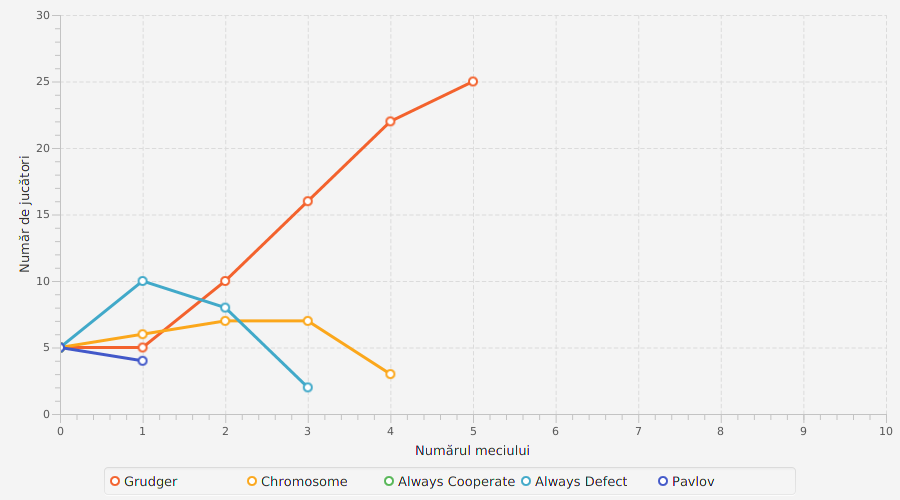
\includegraphics[	
		width=16cm,
		height=7.5cm,
		keepaspectratio
	]{imagini/chart_from_epoch_1528885395051.png}
	\caption{\textit{Evoluția turneului cu eliminare când numărul de runde al meciurilor este 5.}}
	\label{fig:evolutia_cand_numarul_de_runde_este_5}
\end{figure}

\begin{figure}[H]
	\centering
	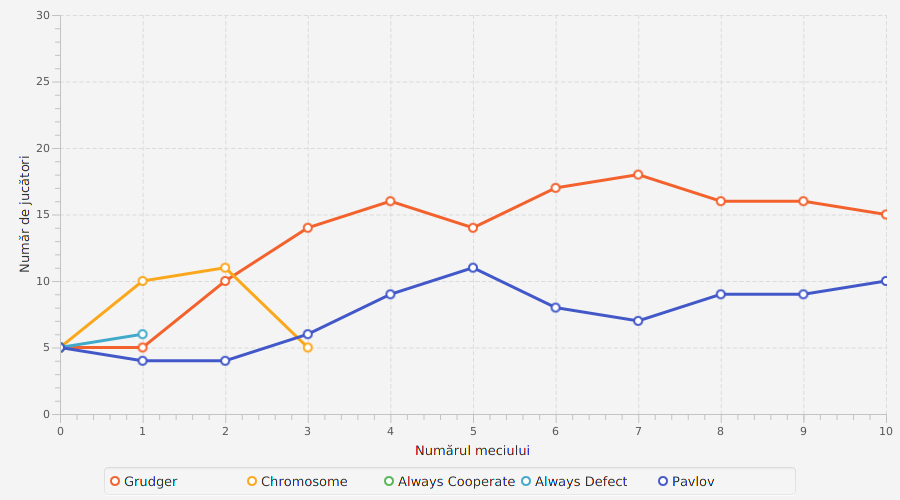
\includegraphics[	
		width=16cm,
		height=7.5cm,
		keepaspectratio
	]{imagini/chart_from_epoch_1528885889300.png}
	\caption{\textit{Evoluția turneului cu eliminare când numărul de runde al meciurilor este 15.}}
	\label{fig:evolutia_cand_numarul_de_runde_este_5}
\end{figure}

Mărind cu 2 numărul de runde din fiecare meci, observăm că strategia propusă de algoritmul genetic câștigă. 

\begin{figure}[H]
	\centering
	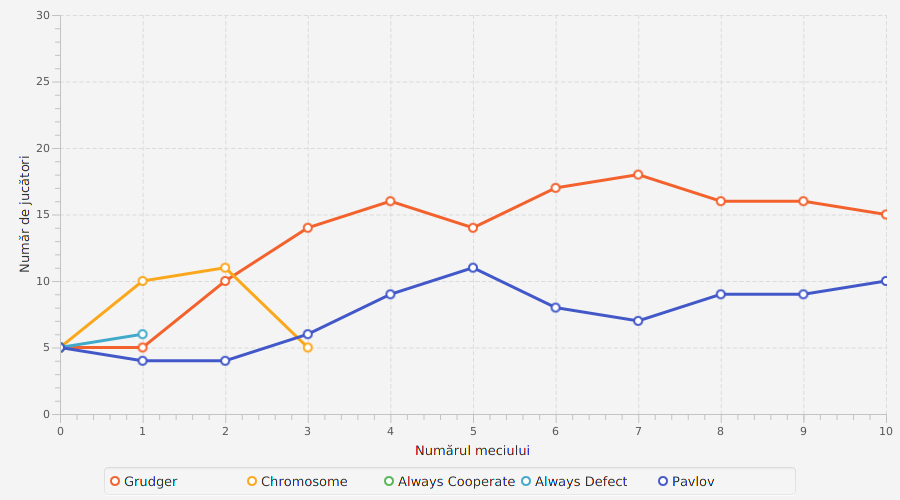
\includegraphics[	
		width=16cm,
		height=7.5cm,
		keepaspectratio
	]{imagini/chart_from_epoch_1528885889300.png}
	\caption{\textit{Evoluția turneului cu eliminare când numărul de runde al meciurilor este 17.}}
	\label{fig:evolutia_cand_numarul_de_runde_este_5}
\end{figure}

Dacă numărul de runde al turneului cu eliminare este mai mare, strategia algoritmului genetic are șanse mai mari de câștig.  
 
\subsection{Probabilitățile de mutație și de încrucișare}

Valorile celor două probabilități nu trebuie să fie foarte mari, deoarece acestea ar putea duce la obținerea unor strategii cu mișcări aleatoare. 

\subsection{Populatia de antrenament}

Consider că o populație diversificată de antrenament poate simula condițiile din faza de testare. Din acest motiv am optat pentru ca aceasta să cuprindă fiecare strategie determinista prezentată la secțiunea de strategii standard (am omis strategia \textbf{Random}). Prezența strategiei \textbf{Random} în faza de antrenament nu ajută la interpretarea calității soluției. Sunt șanse ca acesta strategie nedeterministă să obțină un scor bun în faza de antrenament, însă să nu facă față în faza de testare. 

Am pus câte un individ din fiecare strategie.  










































































































































































































































